% ==================================================================================================
\subsection{Prevalence with and without turnover}
\begin{figure}[H]
  \centering
  \begin{subfigure}{0.45\linewidth}
    \centering\includegraphics[width=\linewidth]{{sit-turnover-prevalence-high-tau=0.1}.pdf}
    \caption{High risk, $\tau=0.1$}
  \end{subfigure}
  \begin{subfigure}{0.45\linewidth}
    \centering\includegraphics[width=\linewidth]{{sit-turnover-prevalence-high-tau=0.2}.pdf}
    \caption{High risk, $\tau=0.2$}
  \end{subfigure}
  \begin{subfigure}{0.45\linewidth}
    \centering\includegraphics[width=\linewidth]{{sit-turnover-prevalence-med-tau=0.1}.pdf}
    \caption{Medium risk, $\tau=0.1$}
  \end{subfigure}
  \begin{subfigure}{0.45\linewidth}
    \centering\includegraphics[width=\linewidth]{{sit-turnover-prevalence-med-tau=0.2}.pdf}
    \caption{Medium risk, $\tau=0.2$}
  \end{subfigure}
  \begin{subfigure}{0.45\linewidth}
    \centering\includegraphics[width=\linewidth]{{sit-turnover-prevalence-low-tau=0.1}.pdf}
    \caption{Low risk, $\tau=0.1$}
  \end{subfigure}
  \begin{subfigure}{0.45\linewidth}
    \centering\includegraphics[width=\linewidth]{{sit-turnover-prevalence-low-tau=0.2}.pdf}
    \caption{Low risk, $\tau=0.2$}
  \end{subfigure}
  \caption{Comparison of projected prevalence for each group
    with and without risk group turnover
    under two different treatment rates $\tau$.
    Note that differences in initial trajectories are attributable
    arbitrary initialization of health states.}
\end{figure}
% ==================================================================================================
\subsection{Rates of transition at equilibrium}
\begin{figure}[H]
  \centering
  \begin{subfigure}{0.31\linewidth}
    \centering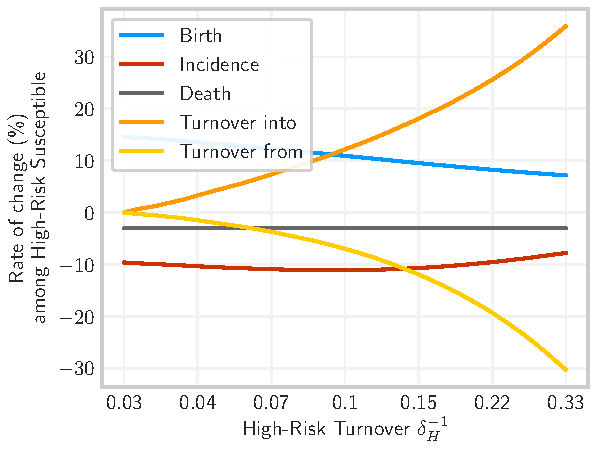
\includegraphics[width=\linewidth]{dX-high-S.pdf}
    \caption{High Risk Susceptible}\label{fig:dX-high-S}
  \end{subfigure}
  \begin{subfigure}{0.31\linewidth}
    \centering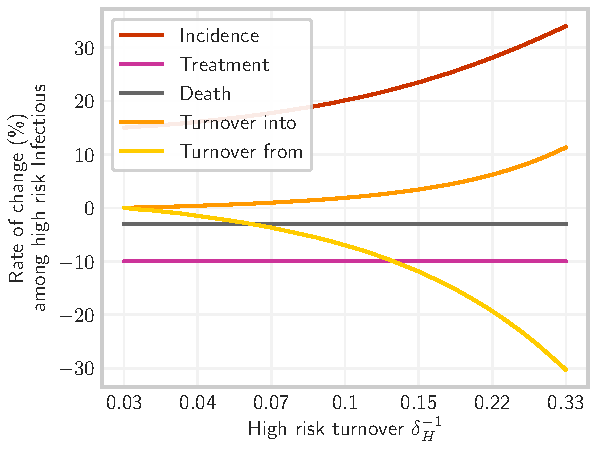
\includegraphics[width=\linewidth]{dX-high-I.pdf}
    \caption{High Risk Infectious}\label{fig:dX-high-I}
  \end{subfigure}
  \begin{subfigure}{0.31\linewidth}
    \centering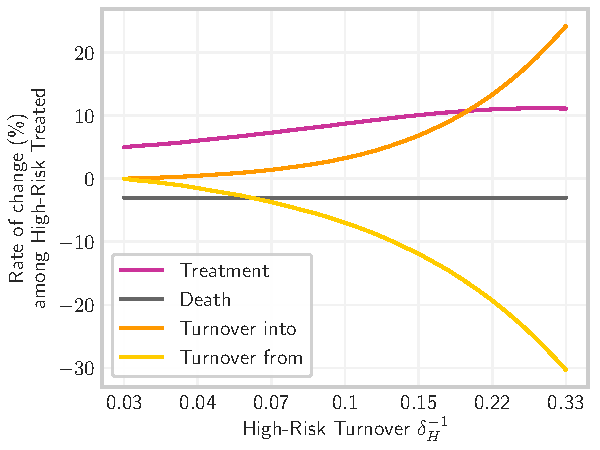
\includegraphics[width=\linewidth]{dX-high-T.pdf}
    \caption{High Risk Treated}\label{fig:dX-high-T}
  \end{subfigure}
  \begin{subfigure}{0.31\linewidth}
    \centering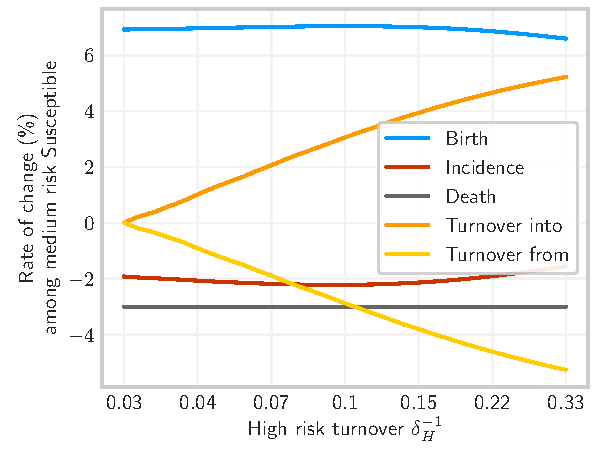
\includegraphics[width=\linewidth]{dX-med-S.pdf}
    \caption{Medium Risk Susceptible}\label{fig:dX-med-S}
  \end{subfigure}
  \begin{subfigure}{0.31\linewidth}
    \centering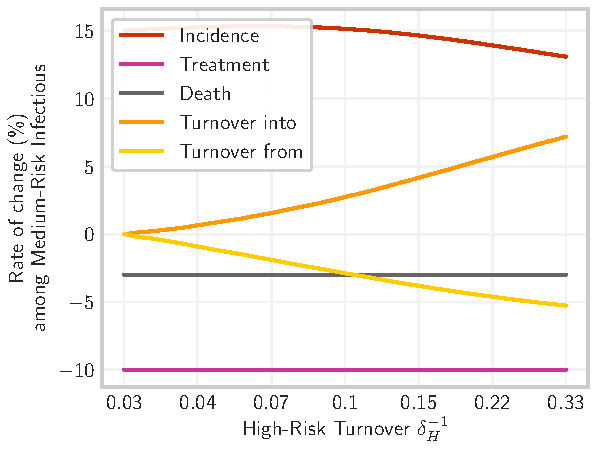
\includegraphics[width=\linewidth]{dX-med-I.pdf}
    \caption{Medium Risk Infectious}\label{fig:dX-med-I}
  \end{subfigure}
    \begin{subfigure}{0.31\linewidth}
    \centering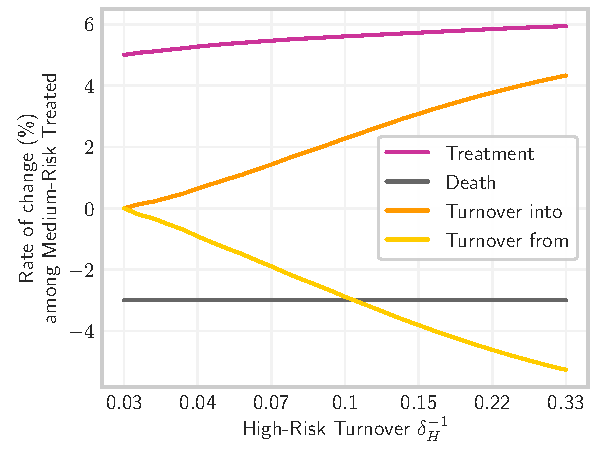
\includegraphics[width=\linewidth]{dX-med-T.pdf}
    \caption{Medium Risk Treated}\label{fig:dX-med-T}
  \end{subfigure}
  \begin{subfigure}{0.31\linewidth}
    \centering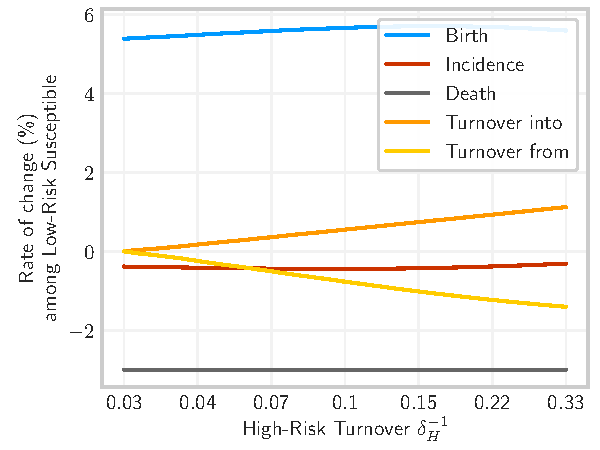
\includegraphics[width=\linewidth]{dX-low-S.pdf}
    \caption{Low Risk Susceptible}\label{fig:dX-low-S}
  \end{subfigure}
  \begin{subfigure}{0.31\linewidth}
    \centering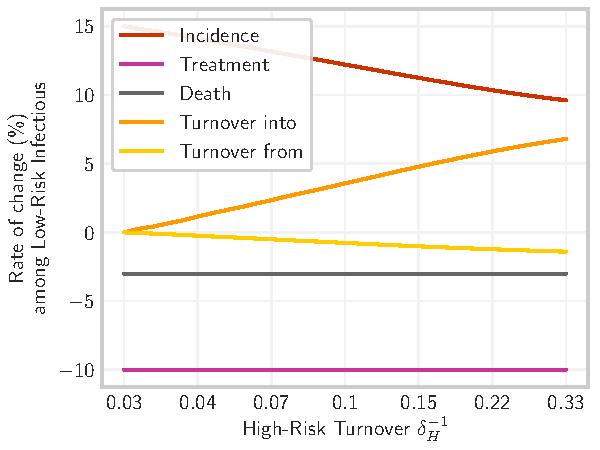
\includegraphics[width=\linewidth]{dX-low-I.pdf}
    \caption{Low Risk Infectious}\label{fig:dX-low-I}
  \end{subfigure}
  \begin{subfigure}{0.31\linewidth}
    \centering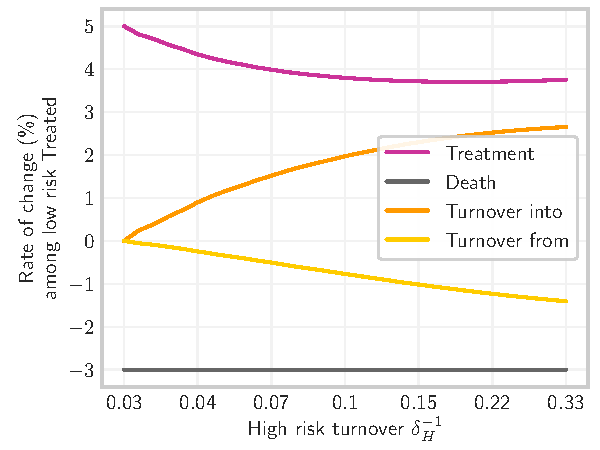
\includegraphics[width=\linewidth]{dX-low-T.pdf}
    \caption{Low Risk Treated}\label{fig:dX-low-T}
  \end{subfigure}
  \caption{Rates of transition among risk groups and health states at equilibrium.
    All transition rates are shown relative to the named group,
    for both afferent and efferent transitions.
    Note that, although each system is at equilibrium,
    profiles should not sum to zero due population growth.}
\end{figure}
\begin{figure}[H]
  \centering\includegraphics[width=0.45\linewidth]{{2d-tip-all-tau=0.1}.pdf}
  \caption{Proportion of new infectious individuals in each risk group
    which are from turnover of infectious individuals,
    as opposed to infection of susceptible individuals in the risk group
    ($\tau = 0.1$).}
  \label{fig:new-inf-L}
\end{figure}
% ==================================================================================================
\subsection{Distribution of health states at equilibrium}
\begin{figure}[H]
  \centering
  \begin{subfigure}{0.45\linewidth}
    \centering\includegraphics[width=\linewidth]{{1d-X-health-high-tau=0.1}.pdf}
    \caption{High Risk}
    \label{fig:}
  \end{subfigure}
  \begin{subfigure}{0.45\linewidth}
    \centering\includegraphics[width=\linewidth]{{1d-X-health-med-tau=0.1}.pdf}
    \caption{Medium risk}
    \label{fig:}
  \end{subfigure}
  \begin{subfigure}{0.45\linewidth}
    \centering\includegraphics[width=\linewidth]{{1d-X-health-low-tau=0.1}.pdf}
    \caption{Low Risk}
    \label{fig:1d-health-low}
  \end{subfigure}
  \begin{subfigure}{0.45\linewidth}
    \centering\includegraphics[width=\linewidth]{{1d-X-health-all-tau=0.1}.pdf}
    \caption{Overall}
    \label{fig:1d-health-all}
  \end{subfigure}
  \caption{Equilibrium incidence ratios between risk groups under different rates of turnover.}
  \label{fig:1d-X-health}
\end{figure}
% ==================================================================================================
\subsection{Equilibrium Incidence and Prevalence Ratios}
\begin{figure}[H]
  \centering
  \begin{subfigure}{0.31\linewidth}
    \centering\includegraphics[width=\linewidth]{{1d-ratio-incidence-high-med-tau=0.1}.pdf}
    \caption{High vs Medium Risk}
    \label{fig:1d-ratio-incidence-high-med}
  \end{subfigure}
  \begin{subfigure}{0.31\linewidth}
    \centering\includegraphics[width=\linewidth]{{1d-ratio-incidence-high-low-tau=0.1}.pdf}
    \caption{High vs Low risk}
    \label{fig:1d-ratio-incidence-high-low}
  \end{subfigure}
  \begin{subfigure}{0.31\linewidth}
    \centering\includegraphics[width=\linewidth]{{1d-ratio-incidence-med-low-tau=0.1}.pdf}
    \caption{Medium vs Low Risk}
    \label{fig:1d-ratio-incidence-med-low}
  \end{subfigure}
  \caption{Equilibrium incidence ratios between risk groups
    under different rates of turnover $\phi$ for a treatment rate $\tau = 0.1$.
    Incidence ratios do not depend on turnover nor treatment
    -- see Eq.~(\ref{eq:foi}).}
  \label{fig:1d-ratio-incidence}
\end{figure}
\begin{figure}[H]
  \centering
  \begin{subfigure}{0.31\linewidth}
    \centering\includegraphics[width=\linewidth]{{1d-ratio-prevalence-high-med-tau=0.1}.pdf}
    \caption{High vs Medium Risk}
    \label{fig:1d-ratio-prevalence-high-med}
  \end{subfigure}
  \begin{subfigure}{0.31\linewidth}
    \centering\includegraphics[width=\linewidth]{{1d-ratio-prevalence-high-low-tau=0.1}.pdf}
    \caption{High vs Low risk}
    \label{fig:1d-ratio-prevalence-high-low}
  \end{subfigure}
  \begin{subfigure}{0.31\linewidth}
    \centering\includegraphics[width=\linewidth]{{1d-ratio-prevalence-med-low-tau=0.1}.pdf}
    \caption{Medium vs Low Risk}
    \label{fig:1d-ratio-prevalence-med-low}
  \end{subfigure}
    \caption{Equilibrium prevalence ratios between risk groups
    under different rates of turnover $\phi$ for a treatment rate $\tau = 0.1$.}
  \label{fig:1d-ratio-prevalence}
\end{figure}
\begin{figure}[H]
  \centering
  \begin{subfigure}{0.31\linewidth}
    \centering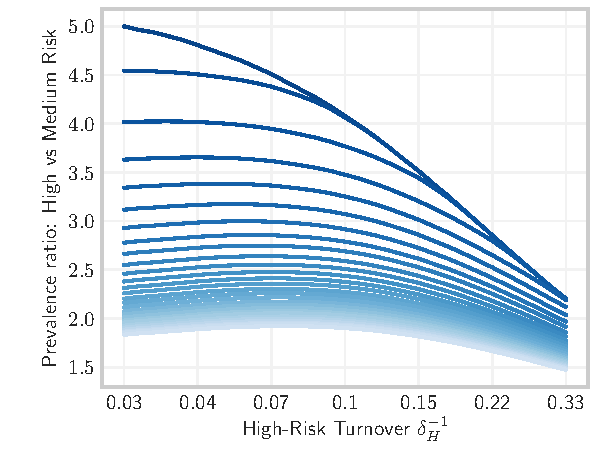
\includegraphics[width=\linewidth]{2d-ratio-prevalence-high-med.pdf}
    \caption{High vs Medium Risk}
    \label{fig:2d-ratio-prevalence-high-med}
  \end{subfigure}
  \begin{subfigure}{0.31\linewidth}
    \centering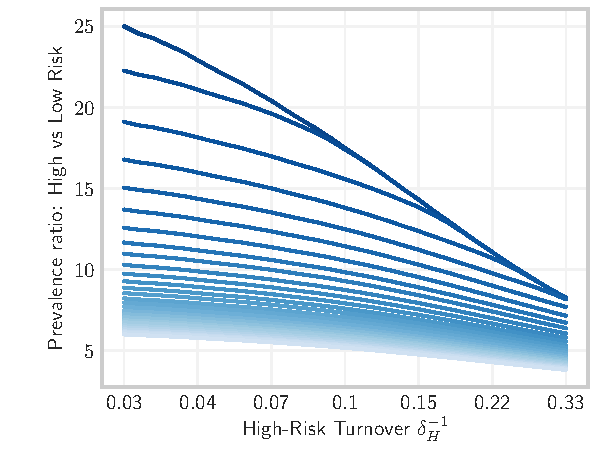
\includegraphics[width=\linewidth]{2d-ratio-prevalence-high-low.pdf}
    \caption{High vs Low risk}
    \label{fig:2d-ratio-prevalence-high-low}
  \end{subfigure}
  \begin{subfigure}{0.31\linewidth}
    \centering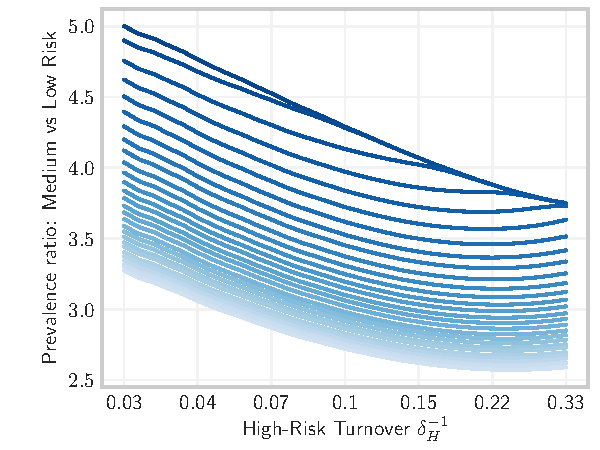
\includegraphics[width=\linewidth]{2d-ratio-prevalence-med-low.pdf}
    \caption{Medium vs Low Risk}
    \label{fig:2d-ratio-prevalence-med-low}
  \end{subfigure}
  \caption{Equilibrium prevalence ratios between risk groups
    under different rates of turnover $\phi$ and treatment $\tau$.
    Turnover increases left to right;
    treatment increases light to dark.}
  \label{fig:2d-ratio-prevalence}
\end{figure}
% ==================================================================================================
\subsection{Equilibrium prevalence before and after model fitting}
\begin{figure}[H]
  \centering
  \begin{subfigure}{0.31\linewidth}
    \centering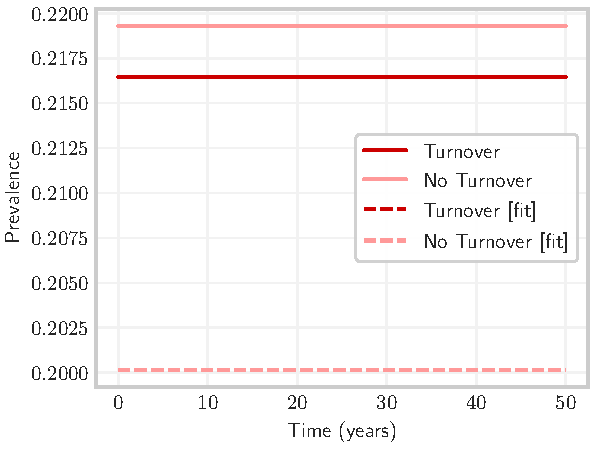
\includegraphics[width=\linewidth]{sit-tpaf-prevalence-high}
    \caption{High risk}
    \label{fig:tpaf-prevalence-high}
  \end{subfigure}
  \begin{subfigure}{0.31\linewidth}
    \centering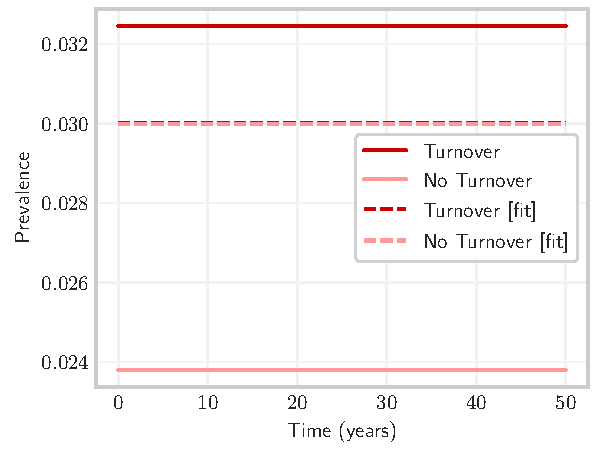
\includegraphics[width=\linewidth]{sit-tpaf-prevalence-low}
    \caption{Low risk}
    \label{fig:tpaf-prevalence-low}
  \end{subfigure}
  \begin{subfigure}{0.31\linewidth}
    \centering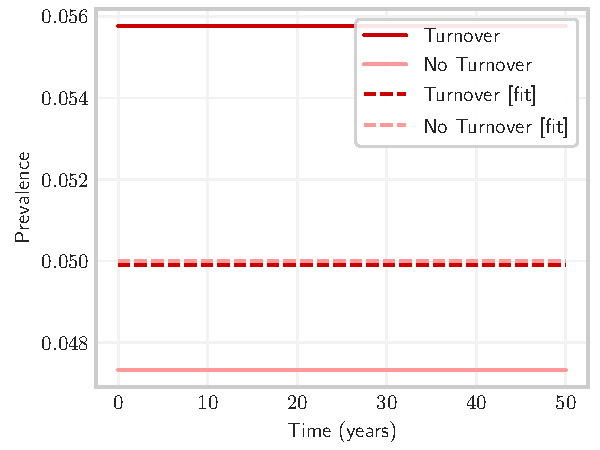
\includegraphics[width=\linewidth]{sit-tpaf-prevalence-all}
    \caption{Overall}
    \label{fig:tpaf-prevalence-all}
  \end{subfigure}
  \caption{Equilibrium prevalence among high and low risk groups as well as overall,
    with and without turnover,
    and with and without fitted $C_i$ to group-specific prevalence.}
  \label{fig:tpaf-prevalence}
\end{figure}
% ==================================================================================================
\subsection{Extreme turnover converges on a homogeneous system}\label{aa:homogenize}
% TODO: update this figure
\begin{figure}[H]
  \centering
  \frame{TODO}: update
%  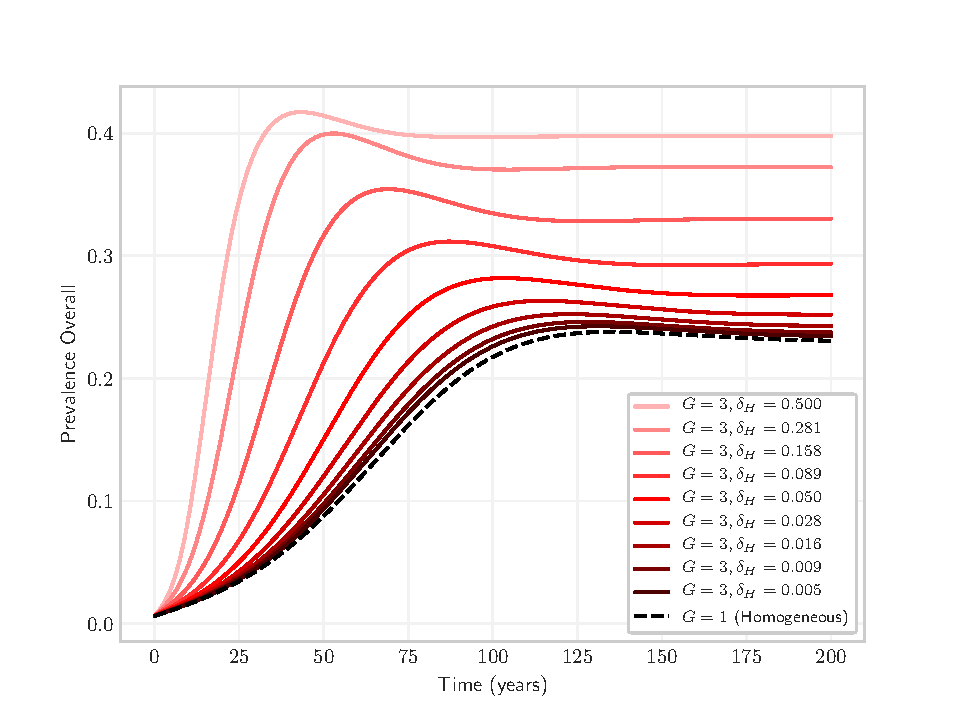
\includegraphics[width=0.6\linewidth]{hetero-converge}
  \caption{Overall prevalence predicted by a heterogeneous system
    for a range of high turnover rates.
    Note how the heterogeneous model ($G = 3$) converges on a homogeneous model ($G = 1$)
    with very high turnover rates.
    Compared to the Base model,
    transmission probability is increased to $\beta = [TBD]$
    in order to yield non-zero equilibrium prevalence in the homogeneous model.}
  \label{fig:hetero-converge}
\end{figure}
% ==================================================================================================
\subsection{``What if'' analysis}\label{aa:what-if}
This section presents hypotheses and preliminary analysis regarding the potential impacts of
alternative model assumptions on the results of Experiment 3.
For reference, Figures~\ref{fig:tpaf-raw-app}~and~\ref{fig:tpaf-fit-app}
show the original results of Experiment 3 (copied from the main text).
\begin{figure}[!tbp]
  \centering
  \begin{subfigure}{0.35\linewidth}
    \centering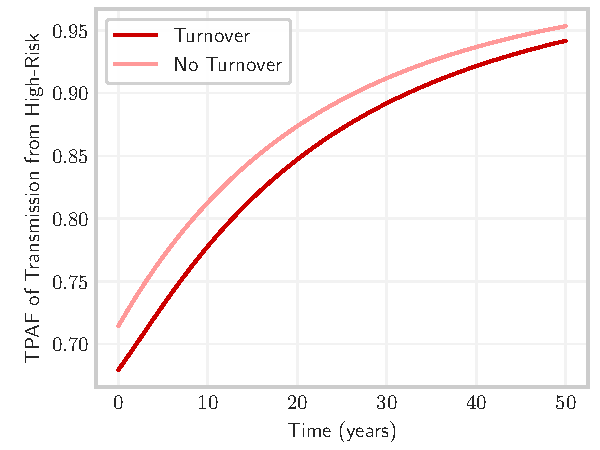
\includegraphics[width=\linewidth]{sit-tpaf-tpaf-high-all-vs=raw}
    \caption{No fitting, original results}
    \label{fig:tpaf-raw-app}
  \end{subfigure}
  \begin{subfigure}{0.35\linewidth}
    \centering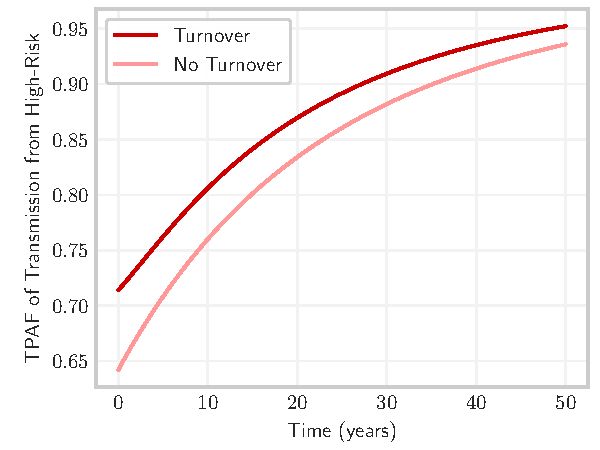
\includegraphics[width=\linewidth]{sit-tpaf-tpaf-high-all-vs=fit}
    \caption{Fitted, original results}
    \label{fig:tpaf-fit-app}
  \end{subfigure}\\
  \begin{subfigure}{0.35\linewidth}
    \centering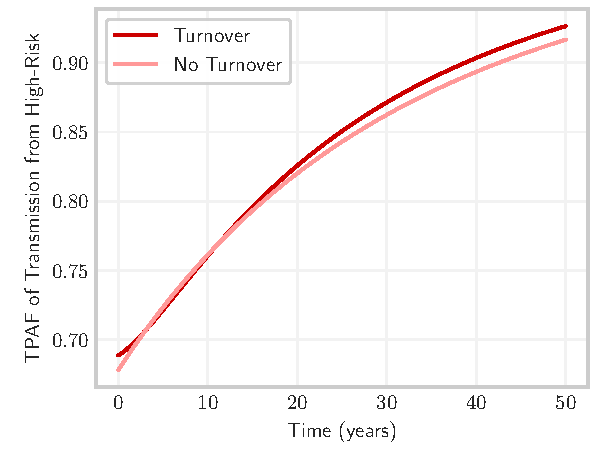
\includegraphics[width=\linewidth]{asso-tpaf-tpaf-high-all-vs=raw}
    \caption{No fitting, assortative mixing}
    \label{fig:tpaf-asso-raw}
  \end{subfigure}
  \begin{subfigure}{0.35\linewidth}
    \centering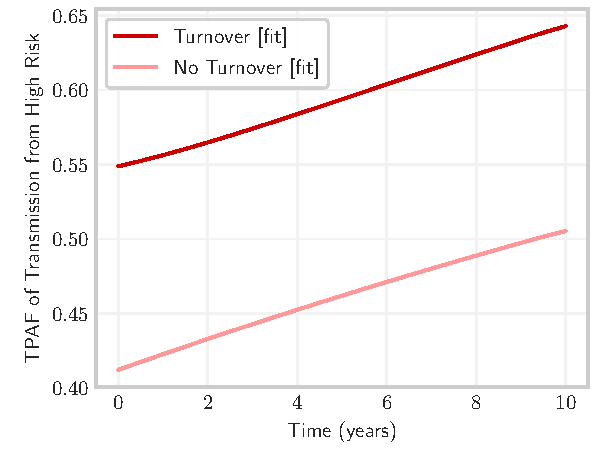
\includegraphics[width=\linewidth]{asso-tpaf-tpaf-high-all-vs=fit}
    \caption{Fitted, assortative mixing}
    \label{fig:tpaf-asso-fit}
  \end{subfigure}\\
  \begin{subfigure}{0.35\linewidth}
    \centering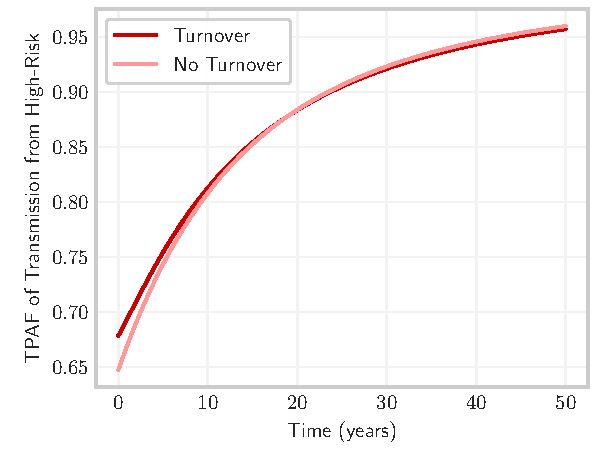
\includegraphics[width=\linewidth]{mort-tpaf-tpaf-high-all-vs=raw}
    \caption{No fitting, disease-attributable mortality}
    \label{fig:tpaf-mort-raw}
  \end{subfigure}
  \begin{subfigure}{0.35\linewidth}
    \centering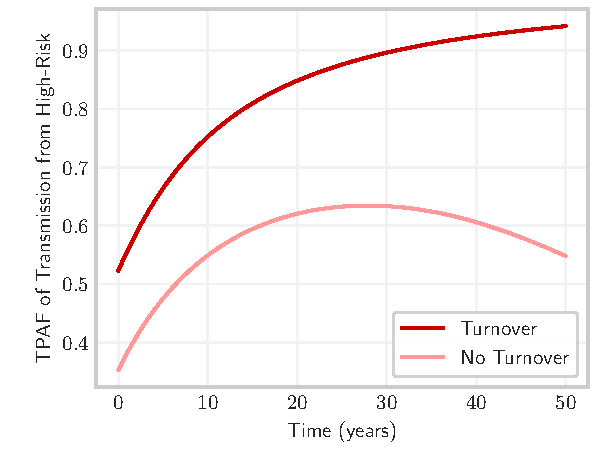
\includegraphics[width=\linewidth]{mort-tpaf-tpaf-high-all-vs=fit}
    \caption{Fitted, disease-attributable mortality}
    \label{fig:tpaf-mort-fit}
  \end{subfigure}\\
  \begin{subfigure}{0.35\linewidth}
    \centering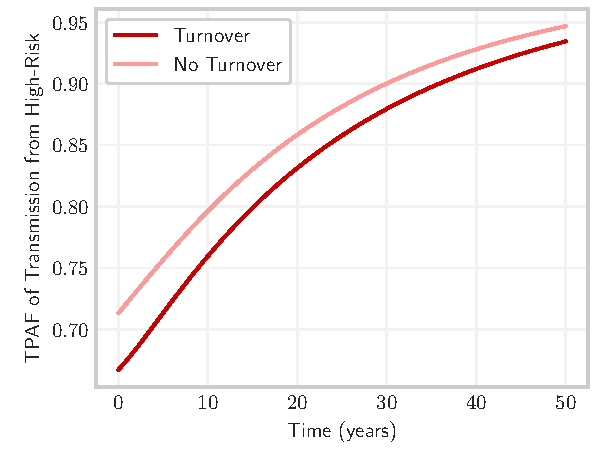
\includegraphics[width=\linewidth]{sirs-tpaf-tpaf-high-all-vs=raw}
    \caption{No fitting, reinfection}
    \label{fig:tpaf-sirs-raw}
  \end{subfigure}
  \begin{subfigure}{0.35\linewidth}
    \centering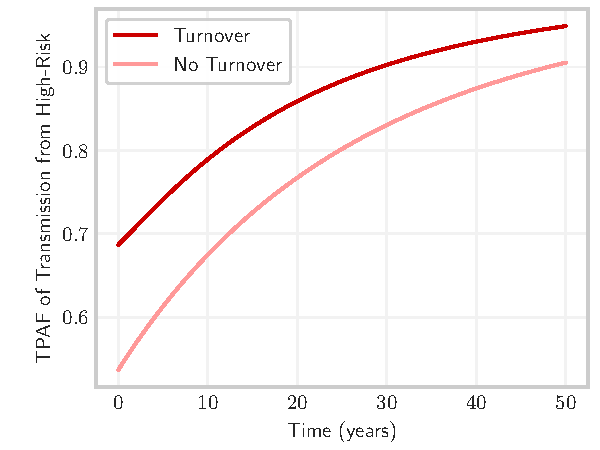
\includegraphics[width=\linewidth]{sirs-tpaf-tpaf-high-all-vs=fit}
    \caption{Fitted, reinfection}
    \label{fig:tpaf-sirs-fit}
  \end{subfigure}
  \caption{TPAF of the high risk group with and without turnover,
    and with and without fitted contact rates to group-specific prevalence.
    Comparison of original results,
    under proportionate mixing,
    with no disease-attributable mortality,
    and without reinfection (a,~b),
    with models considering:
    assortative mixing (c,~d),
    disease-attributable mortality (e,~f),
    and reinfection (g,~h).}
  \label{fig:tpaf-app}
\end{figure}
% --------------------------------------------------------------------------------------------------
\subsubsection{Assortative mixing}\label{aaa:what-if-asso}
Assortative mixing increases the concentration of transmission within the high risk group,
decreasing the TPAF, regardless of turnover.
However, turnover counteracts this effect by
redistributing infectious individuals from high to low risk,
permitting greater onward transmission from
infectious formerly high risk individuals.
Therefore,
while turnover may influence the TPAF of the high risk group through
the STI prevalence before model fitting, and
the inferred risk heterogeneity after model fitting,
we hypothesize that
the secondary effect of turnover to circumvent assortative mixing
would increase the TPAF in both cases.
\par
To explore this hypothesis,
we re-ran Experiment 3 under an assortative mixing scenario,
with $\epsilon = 0.5$ \citep{Nold1980}.
Before model fitting and under assortative mixing
(Figure~\ref{fig:tpaf-asso-raw}),
the TPAF of the high risk group with turnover
is similar to the TPAF without turnover,
whereas under proportional mixing it was lower with turnover than without turnover
(Figure~\ref{fig:tpaf-raw-app}).
After model fitting and under assortative mixing
(Figure~\ref{fig:tpaf-asso-fit}),
the TPAF of the high risk group is even higher with turnover than without turnover,
as compared to proportional mixing
(Figure~\ref{fig:tpaf-fit-app}).
Both of these results support our hypothesis above,
though more comprehensive experiments are needed.
% --------------------------------------------------------------------------------------------------
\subsubsection{Infection-attributable mortality}\label{aaa:what-if-mort}
Disease-attributable mortality disproportionately affects the highest risk group
due to higher infection prevalence.
As a result, the size of the group decreases,%
\footnote{In this case, we assume that no ``market'' forces maintain risk group proportions
  against changes due to unequal death.}
which reduces the TPAF of the group.
Similar to assortative mixing, this reduction in TPAF is again counteracted by turnover,
through re-supply of individuals from lower-risk groups.
Thus, we hypothesize that
while disease-attributable mortality would
decrease the TPAF of the high risk group,
this effect is reduced by turnover,
both before and after model fitting. 
\par
To explore this assertion, we again re-ran Experiment 3,
this time assuming a disease-attributable mortality rate of 0.2 per year
among untreated infected individuals $\mathcal{I}$.
Since establishment of the epidemic was more difficult under these conditions,
we also doubled the probability of transmission per contact $\beta$
from 0.03 to 0.06.
As with assortative mixing,
before model fitting and when disease-attributable mortality is included
(Figure~\ref{fig:tpaf-mort-raw}),
the TPAFs with and without turnover are more similar
than when no disease-attributable mortality is considered
(Figure~\ref{fig:tpaf-raw-app}).
Similarly, after model fitting and when disease attributable mortality is included
(Figure~\ref{fig:tpaf-mort-fit}),
the TPAF of the high risk group is even higher with turnover than without turnover,
as compared to when no disease-attributable mortality is considered
(Figure~\ref{fig:tpaf-fit-app}).
Again, these results support our hypothesis.
% --------------------------------------------------------------------------------------------------
\subsubsection{Reinfection}\label{aaa:what-if-sirs}
\frame{TODO}: update; Figures OK